\boldchapter{Transcription and Replication} %todo{pre-RC and other acronyms}
DNA replication is the biological process that duplicates a cell’s genetic information so that, upon division, daughter cells can inherit a full copy of the genome. 
Replication starts at loci named replication origins. The replisome begins to assemble at these loci during the G1 phase (see below for details) and, upon transition to S-phase, splits into two replicative forks that elongate in opposite directions (fig \ref{fig:repSteps}). 
This process needs to be tightly regulated, as over- or under-replication can lead to severe genome instability. 


While presence of one replication origin is generally sufficient to duplicate prokaryotic genomes, eukaryotic ones are often too large and require multiple origins to be replicated in a timely fashion (i.e. within the confines of S-phase). 
The genome of S.cerevisiae contains 410 confirmed origins (also called ARS, Autonomously Replicating Sequences) \cite{siow:2012:oridb}, but not all of them are used every time the genome is replicated.
Although studies on replication initiation detected discernable patterns in origin specification, studies on single cells have shown that origin selection is not entirely deterministic, but rather a stochastic process \cite{patel:2006:dna, Czajkowsky:2008:dna}. 
This notion raises the question of which elements (either intrinsic to the replication process, or independent of it) can influence origin specification.

In this chapter I will describe what qualifies a replication origin and explore the mechanisms of origin specification in S.cerevisiae, with particular emphasis on the controversial relationship between transcription and DNA replication.

\section{Origins of replication}

Replication origins are cis-acting DNA elements upon which the replisome can assemble and start the replicative process. Because of the stochastic nature of their usage, origins are unlike other cis-acting elements. 
They are collectively required for cell viability, but individually dispensable and redundant \cite{bogenschutz:2014:initiation, dershowitz:2007:linear}. 
This plasticity lessens the selective pressure for any particular origin, as long as the replication process as a whole remains efficient. 


Origins in S.cerevisiae are usually small (100-150 bp), preferentially intergenic, and AT-rich sequences \cite{raghuraman:2016:sequence}. 
Origin-specific motifs are degenerate and generally not conserved. Despite this heterogeneity, several common consensuses were identified as promoters of origin activity and classified as A and B elements\footnote{it should be noted that C elements were also described by celniker and colleagues \cite{celniker:1984:deletion}. However, evidence for the relevance of these motifs \invivo{} is lacking and they will not be discussed here.} (fig \ref{fig:originSchemaIntro}).


\paragraph{A element}
The only essential sequence element, the A element is also called ACS (ARS consensus sequence). 
The ACS is a non-palindromic 11 bp consensus (see fig \ref{fig:originSchemaIntro})\cite{celniker:1984:deletion,nieduszynski:2006:genomewide} that is the binding site of a protein complex called ORC (Origin Recognition Complex). 
Binding of this complex to the origin represents the first step in the replicative process (see below)\cite{diffley:1992:proteindna}.

\begin{figure}[ht]

\centering
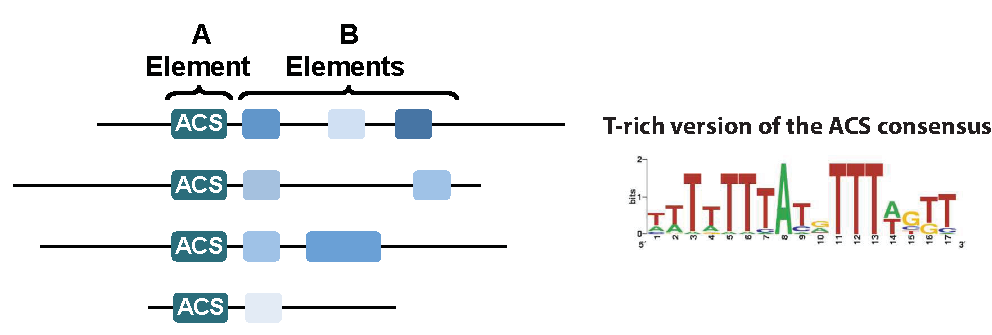
\includegraphics[width=\textwidth]{figures/results/acs}
\caption[ACS consensus and arrangement relative to other origin DNA elements]{Cartoon showing the most typical arrangement of sequence elements within origins. the ACS is required, while several B elements contribute to origin specification dowstream of the T-rich strand of the ACS.}
\label{fig:originSchemaIntro}

\end{figure}

\paragraph{B elements}
A family of motifs with little sequence conservation, B elements are mainly AT-rich and always map downstream of the T-rich strand of the ACS (fig \ref{fig:originSchemaIntro})\cite{raghuraman:2016:sequence}. 
While a match to the A element consensus is found in every origin \cite{celniker:1984:deletion}, no individual B element is universally required for origin activity \cite{marahrens:1992:yeast,lucas:2003:dynamics}. Collectively, however, B elements constitute a requirement for proper origin activity.

B elements were originally thought to facilitate DNA unwinding due to their AT-richness \cite{huang:1993:dna}. Subsequent studies, however, revealed that some B elements are playing a more active role, contributing to the recruitment of the replisome \cite{wilmes:2002:b2}.


\vspace{5mm}

Sequence elements are not enough to qualify an active origin. 
More than 10,000 matches for the ACS exist in the genome of S.cerevisiae, however, only 400 replication origins were identified. 
Moreover, it has been reported that some origins are able to efficiently drive replication of a plasmid, but are rarely used \invivo{} \cite{newlon:1993:analysis, santocanale:1999:activation}. 
Investigation of this context-dependent activity showed that nucleosome positioning plays a crucial role in origin activity and that functional origins are always associated with Nucleosome Free Regions. 
In support of this notion, experiments forcing nucleosome assembly within the A or B elements resulted in abrogation of replisome assembly \cite{lipford:2001:nucleosomes}. 


The ACS itself was speculated to be able to drive nucleosome positioning, a notion supported by \invivo{} studies \cite{eaton:2010:conserved, berbenetz:2010:diversity}.
In these reports, the authors show that ACS sequences contained in active origins are surrounded by NFR, although formation of the latter is per se not sufficient to specify an origin as non-functional ACS are also associated with low nucleosome occupancy, albeit to a lesser extent.


Lastly, binding sites for transcription factors were detected within origins and, although their function remains somewhat unclear, are speculated to contribute to the maintenance of NFR within the origin \cite{diffley:1992:proteindna, rhode:1989:gene}. 
For example, the transcription factor Abf1 (ARS Binding Factor) is often found near origins and is known to recruit chromatin remodeling complexes to deplete nucleosomes at promoter regions. 
Studies on these origins showed that deleting Abf1 binding sites results in loss of activity, but replacing the sites with those of other transcription factors associated with NFR generation, such as Rap1, retains the replication activity \cite{marahrens:1992:yeast}.


\section{Mechanisms of DNA replication}

Because of the importance of proper DNA replication for genome stability, its mechanism of action must ensure that the entirety of the genome is duplicated once and only once. 
In order to achieve this result, replication occurs in two discrete steps \cite{diffley:1994:two}.
The first step occurs exclusively in the G1-phase, and is called origin licensing.
During this step the six subunits Origin Recognition Complex (ORC) binds the ACS and associates with two ancillary factors named Cdc6 and Cdt1. 
When interacting, these three licensing factors are able to recruit multiple pairs of inactive replicative helicases around double stranded DNA, forming the pre-replication complex (Fig \ref{fig:repSteps})\cite{gambus:2011:mcm27, remus:2009:concerted, seki:2000:stepwise, rowles:1999:changes, donovan:1997:cdc6pdependent}.
Replicative helicases are multisubunit complexes composed of MiniChromosome Maintenance proteins (MCM2 to MCM7). 
In S-phase, MCM2-7 will serve both as platforms for the assembly of other replisome components and as driving force for replicative fork elongation. 
It is important to note that during the first step of replication, only a subset of all origins are licensed. This subset is influenced by specific origin properties (e.g. strength of the ORC binding site, nucleosome occupancy etc.), but not deterministically chosen.

\begin{figure}[ht]

\centering
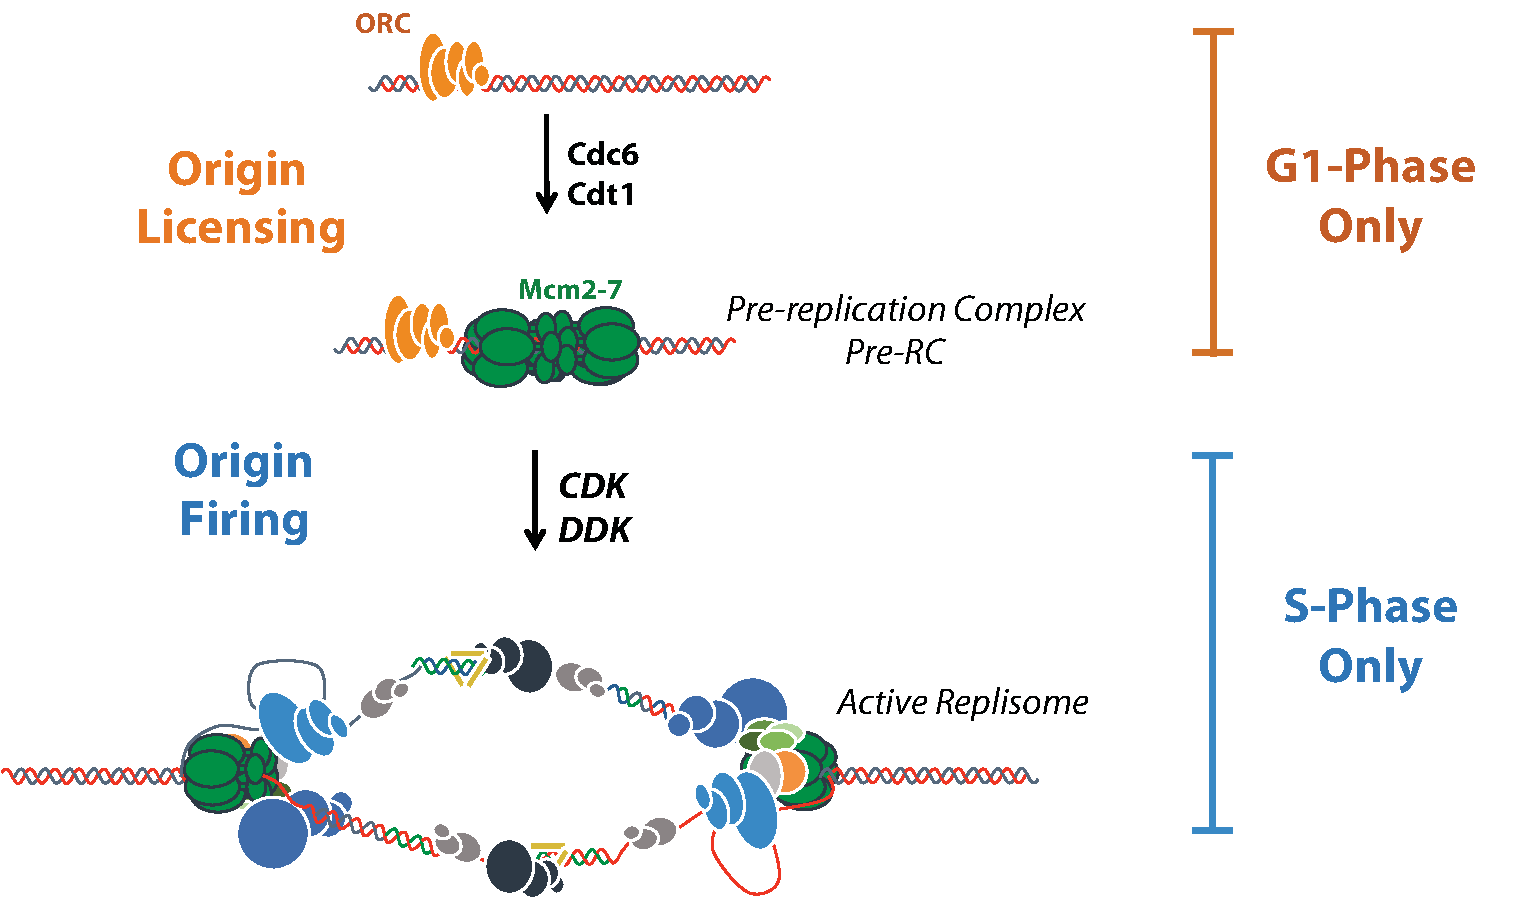
\includegraphics[width=\textwidth]{figures/introduction/repSteps}
\caption[Stepwise mechanism of DNA replication]{DNA replication takes place in two distinct steps. First ORC is required to bind to replication origins during the G1-phase and recruit the Pre-replication complex. Second, upon entry in S-phase, the pre-RC (among others) is phosphorylated and the full replisome can assemble and eventually fire.}
\label{fig:repSteps}

\end{figure}

The end of the G1-phase and the beginning of the S-phase marks the end of the licensing step and the beginning of the second step of DNA replication: the activation step. 
During this step, dormant pre-replication complexes at licensed origins activate, assemble into the active replisome and eventually fire. 
In order to prevent re-licensing of an already activated origin—and therefore avoid the risk of firing the same origin twice, leading to re-replication—the ORC complex is  inhibited through phosphorylation and MCM2-7 are rapidly depleted from the nucleus before this step begins \cite{nguyen:2001:cyclindependent}. 


Entry into S-phase coincides with a cascade of phosphorylation signals that activates the CDK and DDK kinase complexes. 
These cell cycle specific enzymes phosphorylate the pre-replication complex and are thought to induce structural rearrangements that allow assembly of the complete replisome. 
First the replicative helicases form the CMG complex (Cdc45-MCM-GINS) with Cdc45 and the GINS complex \cite{moyer:2006:isolation, aparicio:2009:human}. 
Subsequently, DNA polymerases pol $\delta$ and $\epsilon$ join the forming replisome. 
This allows the complete replisome to form and marks the start of fork elongation.


\section{Transcription and origin usage}

Multiple factors can affect the efficiency of an origin.  
For example, sequence elements can strongly contribute by affecting either ORC binding or pre-RC assembly. 
However, extrinsic factors such as nucleosome positioning can epistatically affect origin activity by occluding said elements \cite{bodmerglavas:2001:rna}. 
This raises the question: what other extrinsic processes can impact the initiation of replication? Several studies have investigated the effects of transcription on origin activity, but the results in the literature are controversial. 
While it generally agreed upon that transcription has a deleterious effect on origin activity \cite{tanaka:1994:transcription,nieduszynski:2005:requirement}, a substantial amount of evidence exist to argue that presence of RNAPII within origins can enhance their activity \cite{yankulov:1999:mcm,gauthier:2002:role}. 


Tanaka and colleagues originally investigated the problem by analyzing ARS1, an origin that partially overlaps with the gene TRP1. 
They observed that changing the endogenous promoter of TRP1 to a stronger one led to significant loss of origin activity \cite{tanaka:1994:transcription}.
A later study found that high transcriptional output across origins increases their sensitivity to ORC mutants (i.e. transcription increases loss of activity in the context of ORC mutations). 
The authors proposed a model according to which susceptibility to ORC mutants strictly depends on the intrinsic properties of each origin (e.g. sequence elements) but can be affected by extrinsic elements such as transcription \cite{nieduszynski:2005:requirement}. 


In seeming contradiction, several other studies demonstrated how RNAPII is capable of enhancing origin activity through its presence in the vicinity of the origin. 
In particular, the CTD of RNAPII was shown to interact with subunits of the replicative helicase MCM2-7 in both xenopus and human \cite{yankulov:1999:mcm}. 
Studies in yeast corroborated this result by showing that not only tethering of RNAPII CTD at replication origins can enhance activity, but also that cells with a shortened CTD (10 heptapeptide motifs in place of 26) show increased plasmid loss rates \cite{gauthier:2002:role}. 
Lastly, a recent study investigated origins associated with rDNA loci and concluded that RNAPII molecules participate to ORC binding to origins through their  ser2-Phosphorylated CTD \cite{mayan:2013:rnapii}. 


Although there are compelling arguments on both sides, mechanistic details are still lacking and current models cannot yet account for these discrepancies.










